\documentclass{standalone}
\usepackage{tikz}
\usetikzlibrary{shapes.geometric}
\begin{document}
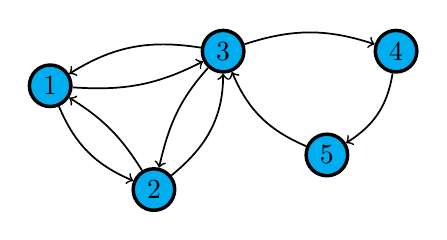
\begin{tikzpicture}
[every node/.style={inner sep=0pt}]
\node (1) [circle, minimum size=15.0pt, fill=cyan, line width=1.25pt, draw=black] at (50.0pt, -37.5pt) {\textcolor{black}{1}};
\node (2) [circle, minimum size=15.0pt, fill=cyan, line width=1.25pt, draw=black] at (87.5pt, -75.0pt) {\textcolor{black}{2}};
\node (3) [circle, minimum size=15.0pt, fill=cyan, line width=1.25pt, draw=black] at (112.5pt, -25.0pt) {\textcolor{black}{3}};
\node (5) [circle, minimum size=15.0pt, fill=cyan, line width=1.25pt, draw=black] at (150.0pt, -62.5pt) {\textcolor{black}{5}};
\node (4) [circle, minimum size=15.0pt, fill=cyan, line width=1.25pt, draw=black] at (175.0pt, -25.0pt) {\textcolor{black}{4}};
\draw [line width=0.625, ->, color=black] (1) to  [in=157, out=293] (2);
\draw [line width=0.625, ->, color=black] (2) to  [in=270, out=39] (3);
\draw [line width=0.625, ->, color=black] (3) to  [in=32, out=171] (1);
\draw [line width=0.625, ->, color=black] (1) to  [in=207, out=356] (3);
\draw [line width=0.625, ->, color=black] (3) to  [in=77, out=228] (2);
\draw [line width=0.625, ->, color=black] (2) to  [in=328, out=122] (1);
\draw [line width=0.625, ->, color=black] (3) to  [in=162, out=18] (4);
\draw [line width=0.625, ->, color=black] (4) to  [in=32, out=261] (5);
\draw [line width=0.625, ->, color=black] (5) to  [in=293, out=157] (3);
\end{tikzpicture}

\end{document}
